\documentclass[11pt,a4paper]{article}
\usepackage[T1]{fontenc}
\usepackage[margin=2.3cm]{geometry}
\usepackage{amsmath,amssymb}
\usepackage{graphicx}
\usepackage[dvipsnames]{xcolor}
\usepackage{enumitem}
\usepackage[colorlinks=true,linkcolor=blue,urlcolor=blue]{hyperref}
\setlength{\parskip}{0.6em}
\setlength{\parindent}{0pt}
\begin{document}

\begin{center}{\LARGE\bfseries openfractal}\\[0.4em]{\large Render a Mandelbrot and Julia zoom from complex numbers, in three sessions.}\\[0.2em]\small PAN IIT OSS explainer \textbullet{} secondary school to diploma / undergraduate (levels 3-5)\end{center}

\section*{Why this exists}
Every fractal zoom video is the same question asked millions of times: does this number run away under one simple rule? This explainer shows the mathematics behind that, using only complex numbers and a loop, so you can build it yourself.

\section*{The end goal}
Render a Mandelbrot and Julia zoom video from complex numbers. The end goal is a Mandelbrot and Julia zoom video made from complex numbers. The same ideas (iteration, escape, numerical precision) appear in dynamical systems, root finding and chaos.

\section*{How the three sessions build up}
\begin{enumerate}[nosep]
\item \textbf{Session 1: Complex numbers are points that move, and some escape} (Level 1, conceptual interactive model, 60 min).
\item \textbf{Session 2: Modulus, argument and the escape-time algorithm} (Level 2, mathematical engineering model, 75 min).
\item \textbf{Session 3: A fast renderer: smooth colour, area and the limits of floating point} (Level 3, simulation and validation, 90 min).
\end{enumerate}

\section{Session 1: Complex numbers are points that move, and some escape}

\subsection*{A. Real-world problem}
Every fractal picture and zoom video is built from one yes/no question asked for each pixel: if I keep applying the same rule, does the number run away? To ask it we need numbers that live on a plane, because a picture is a plane. Complex numbers are exactly that: a number with two parts, so one number is one point. Can we tell, just by repeating z -\textgreater{} z\textasciicircum{}2 + c a few times, which values of c are tame and which run away?

\subsection*{B. Concept and theory}
A complex number is z = a + b i, where a is the real part, b is the imaginary part and i is a new number with i * i = -1. We draw it as the point (a, b). Adding two complex numbers adds the real parts and the imaginary parts, which slides the point. Multiplying by i sends a + b i to -b + a i: the point is turned by 90 degrees about 0, and after four turns it is back where it started. The rule z -\textgreater{} z\textasciicircum{}2 + c is applied again and again from z0 = 0; the list z0, z1, z2, ... is the orbit of c. If the distance \textbar{}z\textbar{} from 0 ever exceeds 2 we say the orbit escapes (Session 2 shows why 2 is the right line); otherwise it stays.

\begin{itemize}[nosep]
\item z: a complex number a + b i, a point (a, b) (no unit)
\item c: the fixed constant of the rule (no unit)
\item z\_k: the orbit after k steps (z\_0 = 0) (no unit)
\item \textbar{}z\textbar{}: distance of z from 0, sqrt(a\textasciicircum{}2 + b\textasciicircum{}2) (no unit)
\item k: step number (count)
\end{itemize}

\begin{equation*}
z=a+bi,\qquad i^2=-1
\end{equation*}

\begin{equation*}
(a+bi)+(c+di)=(a+c)+(b+d)i
\end{equation*}

\begin{equation*}
i\,(a+bi)=-b+ai\quad\text{(a quarter turn about }0\text{)}
\end{equation*}

\begin{equation*}
z_{k+1}=z_k^2+c,\qquad z_0=0
\end{equation*}

\begin{center}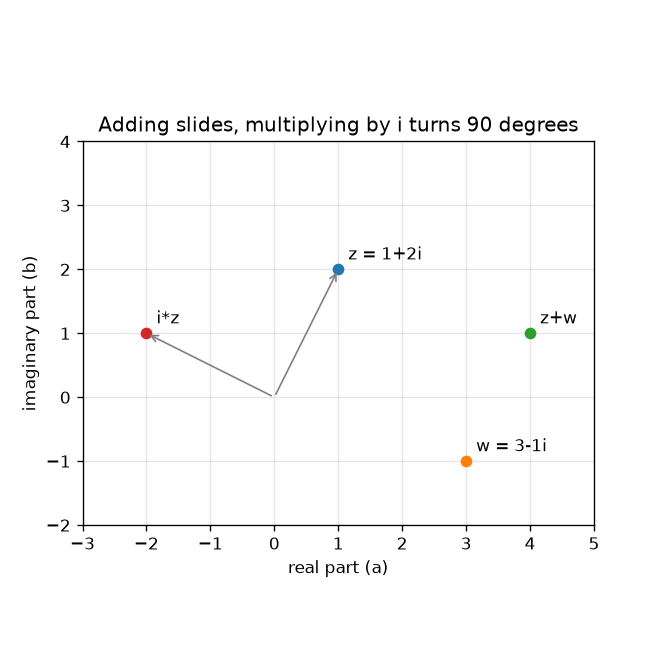
\includegraphics[width=0.85\linewidth]{figures/s01_plane_moves.png}\\\small Adding slides a point; multiplying by i turns it by 90 degrees about 0.\end{center}

\subsection*{E. Worked example}
For c = 0.5 + 0.5i, find z1 to z5 and the step at which the orbit escapes.
\begin{enumerate}[nosep]
\item z1 = 0*0 + c = 0.5 + 0.5i.
\item z2 = z1\textasciicircum{}2 + c. Now (0.5 + 0.5i)\textasciicircum{}2 = 0.25 + 0.5i + 0.25 i\textasciicircum{}2 = 0.5i, so z2 = 0.5 + 1.0i.
\item z3 = (0.5 + 1.0i)\textasciicircum{}2 + c = (0.25 - 1 + 1.0i) + c = -0.75 + 1.0i + 0.5 + 0.5i = -0.25 + 1.5i.
\item z4 = (-0.25 + 1.5i)\textasciicircum{}2 + c = (0.0625 - 2.25 - 0.75i) + c = -2.1875 - 0.75i + 0.5 + 0.5i = -1.6875 - 0.25i, with \textbar{}z4\textbar{} = 1.706 (still within 2).
\item z5 = (-1.6875 - 0.25i)\textasciicircum{}2 + c = (2.8477 - 0.0625 + 0.84375i) + c = 3.2852 + 1.3438i, with \textbar{}z5\textbar{} = 3.549 \textgreater{} 2.
\end{enumerate}
\textbf{Answer.} z1 = 0.5 + 0.5i, z2 = 0.5 + 1.0i, z3 = -0.25 + 1.5i, z4 = -1.6875 - 0.25i, z5 = 3.285 + 1.344i; the orbit escapes at step 5.

\subsection*{F. Questions}
\begin{enumerate}[nosep]
\item \textbf{Conceptual.} Why does multiplying by i turn a point by a quarter turn and never change its distance from 0?
\item \textbf{Numerical.} For c = 1 compute z1, z2, z3 and z4 by hand. At which step does the orbit first have distance above 2? Give the distances.
\item \textbf{Graph and simulation interpretation.} In the distance graph for c = -1, what pattern do you see, and why does the orbit never escape?
\item \textbf{Design and optimisation challenge.} Design: on the real axis (c with zero imaginary part), find by experiment the largest c for which the orbit still stays within 2 for 50 steps, to two decimal places, and the smallest negative c that does. What do you notice about the stay set?
\end{enumerate}

\section{Session 2: Modulus, argument and the escape-time algorithm}

\subsection*{A. Real-world problem}
To draw the picture we must decide, for tens of thousands of pixels, whether an orbit escapes, and a computer cannot iterate for ever. How far must it go? Why is 2 the point of no return? And what is the difference between the Mandelbrot picture and a Julia picture, when both come from the same rule z -\textgreater{} z\textasciicircum{}2 + c? Finally, the practical question: when we zoom in, how many iterations do we need so that the boundary of the set is not smeared?

\subsection*{B. Concept and theory}
A complex number has a modulus \textbar{}z\textbar{} (distance from 0) and an argument arg z (angle from the real axis). Multiplying two numbers multiplies the moduli and adds the arguments; so squaring squares the modulus and doubles the angle, and the rule z -\textgreater{} z\textasciicircum{}2 + c is 'square and double, then slide by c'. The escape-time algorithm iterates the rule until \textbar{}z\textbar{} \textgreater{} 2 or a limit max\_iter is reached and returns the number of steps used. Why 2: if \textbar{}c\textbar{} \textless{}= 2 and \textbar{}z\textbar{} \textgreater{} 2 then \textbar{}z\textasciicircum{}2 + c\textbar{} \textgreater{}= \textbar{}z\textbar{}\textasciicircum{}2 - 2 = \textbar{}z\textbar{} + (\textbar{}z\textbar{} - 2)(\textbar{}z\textbar{} + 1) \textgreater{} \textbar{}z\textbar{} + 3(\textbar{}z\textbar{} - 2), so the distance grows at least by a fixed positive amount every step and the orbit leaves for ever; if \textbar{}c\textbar{} \textgreater{} 2 then z1 = c is already beyond 2. The Mandelbrot set M is the set of c for which the orbit of z0 = 0 stays bounded; it lies inside the disc \textbar{}c\textbar{} \textless{}= 2. The (filled) Julia set of a fixed c is the set of starting values z0 whose orbit stays bounded; it is in one connected piece exactly when c is in M (a known fact we state without proof). Near the boundary orbits take long to escape, so with a finite max\_iter some escaping pixels are wrongly painted inside.

\begin{itemize}[nosep]
\item \textbar{}z\textbar{}: modulus: distance of z from 0 (no unit)
\item arg z: argument: angle of z from the positive real axis (degrees)
\item c: the constant of the rule (the pixel in a Mandelbrot picture) (no unit)
\item z0: starting value (the pixel in a Julia picture) (no unit)
\item max\_iter: iteration limit of the algorithm (steps)
\item w: window width in the picture (same unit as c)
\item error: share of pixels painted inside that escape later (fraction)
\end{itemize}

\begin{equation*}
|zw|=|z|\,|w|,\qquad \arg(zw)=\arg z+\arg w
\end{equation*}

\begin{equation*}
|z^2+c|\ \ge\ |z|^2-|c|\ \ge\ |z|+(|z|-2)(|z|+1)\quad(|z|>2,\ |c|\le 2)
\end{equation*}

\begin{equation*}
M=\{c:\ z_0=0,\ z_{k+1}=z_k^2+c\ \text{stays bounded}\}
\end{equation*}

\begin{equation*}
J_c=\{z_0:\ z_{k+1}=z_k^2+c\ \text{stays bounded}\}
\end{equation*}

\begin{center}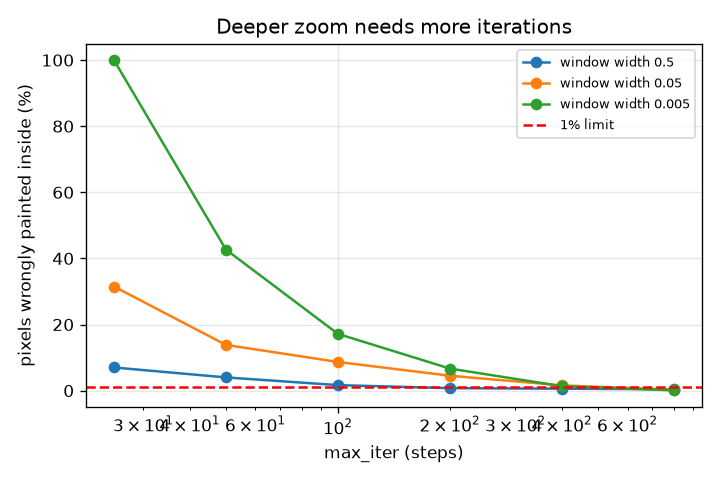
\includegraphics[width=0.85\linewidth]{figures/s02_iterations_needed.png}\\\small Share of wrongly-inside pixels against max\_iter for three window widths at the seahorse valley.\end{center}

\subsection*{E. Worked example}
For z = 3 + 4i and w = 1 + i, find the modulus and argument of z, w and z*w, and check the multiplication rule.
\begin{enumerate}[nosep]
\item \textbar{}z\textbar{} = sqrt(3\textasciicircum{}2 + 4\textasciicircum{}2) = 5 and arg z = atan2(4, 3) = 53.13 degrees.
\item \textbar{}w\textbar{} = sqrt(2) = 1.414 and arg w = 45 degrees.
\item z * w = (3 + 4i)(1 + i) = 3 + 3i + 4i + 4 i\textasciicircum{}2 = -1 + 7i.
\item \textbar{}z w\textbar{} = sqrt(1 + 49) = sqrt(50) = 7.071, and \textbar{}z\textbar{} \textbar{}w\textbar{} = 5 * 1.414 = 7.071. They agree.
\item arg(z w) = atan2(7, -1) = 98.13 degrees, and arg z + arg w = 53.13 + 45 = 98.13 degrees. They agree.
\end{enumerate}
\textbf{Answer.} \textbar{}z\textbar{} = 5, arg z = 53.13 degrees; \textbar{}w\textbar{} = 1.414, arg w = 45 degrees; z*w = -1 + 7i with modulus 7.071 and argument 98.13 degrees.

\subsection*{F. Questions}
\begin{enumerate}[nosep]
\item \textbf{Conceptual.} Why is it safe to stop iterating as soon as \textbar{}z\textbar{} \textgreater{} 2, but not safe to conclude 'stays' after any finite number of steps?
\item \textbf{Numerical.} Compute \textbar{}z\textasciicircum{}2\textbar{} and arg(z\textasciicircum{}2) for z = 3 + 4i, from the modulus and argument. Check by multiplying out.
\item \textbf{Graph and simulation interpretation.} In the iteration-error graph, why does each curve fall, and why is the curve for width 0.005 above the curve for width 0.5 at max\_iter = 100?
\item \textbf{Design and optimisation challenge.} Design: a zoom video moves from width 0.5 to width 0.005 at the seahorse valley. Choose max\_iter for the first and last frame from the ladder 25, 50, 100, 200, 400, 800 with at most 1 percent wrong pixels, and say what you would do in between.
\end{enumerate}

\section{Session 3: A fast renderer: smooth colour, area and the limits of floating point}

\subsection*{A. Real-world problem}
A zoom video needs hundreds of frames, so a Python loop over pixels is hopeless; and a picture coloured by integer counts shows ugly bands. How do we make the renderer fast and smooth? And how do we know a renderer is right, when the true picture is infinitely complicated? Finally, every zoom video has a limit: somewhere around a magnification of 10\textasciicircum{}13 the picture turns into blocks. Where exactly, and why?

\subsection*{B. Concept and theory}
The vectorised renderer keeps every pixel's z in one array and does z = z*z + c for all unfinished pixels at once, removing a pixel from the list when \textbar{}z\textbar{} exceeds a large bailout radius (256). The work is counted as the total number of z-updates. The integer escape count n gives colour bands; the continuous count nu = n + 1 - log2(ln\textbar{}z\_n\textbar{}) interpolates between them, because near the escape \textbar{}z\textbar{} roughly squares each step, so ln\textbar{}z\textbar{} doubles and log2 of it measures the fraction of a step; nu hardly changes with the bailout radius. To check the renderer we use known points (c = 0 inside, c = 1 outside, c = -1 periodic, c = -2 on the boundary and still inside, c = -2.0001 outside) and the area of M: for N random points in the upper half-box [-2, 0.5] x [0, 1.15] with a fraction p inside, area = 2 * 2.875 * p, with statistical error 2 * 2.875 * sqrt(p (1 - p) / N), which falls like 1/sqrt(N); a finite max\_iter makes the estimate slightly too large. The literature value of the area is about 1.5066. Finally, a float64 number carries about 16 significant digits, so near x = -0.74 neighbouring floats are about 1.1e-16 apart; when the pixel spacing w/nx approaches that, neighbouring pixels get the same coordinate.

\begin{itemize}[nosep]
\item n: first step with \textbar{}z\textbar{} above the bailout (integer escape count) (steps)
\item nu: continuous (smooth) escape count (steps)
\item work: total number of z-updates performed (updates)
\item N: number of random sample points (count)
\item p: fraction of sample points that look inside (fraction)
\item A: area of the Mandelbrot set (square units of the c plane)
\item w: window width (same unit as c)
\item nx: image width in pixels (pixels)
\end{itemize}

\begin{equation*}
\nu=n+1-\log_2\!\big(\ln |z_n|\big)
\end{equation*}

\begin{equation*}
A\approx 2\,A_{\mathrm{box}}\,p,\qquad A_{\mathrm{box}}=2.5\times1.15=2.875
\end{equation*}

\begin{equation*}
\sigma_A=2\,A_{\mathrm{box}}\sqrt{\frac{p(1-p)}{N}}
\end{equation*}

\begin{equation*}
\text{pixels collapse when }\ \frac{w}{n_x}\ \lesssim\ \varepsilon_{\mathrm{mach}}\,|x|\approx 1.1\times10^{-16}\times 0.74
\end{equation*}

\begin{center}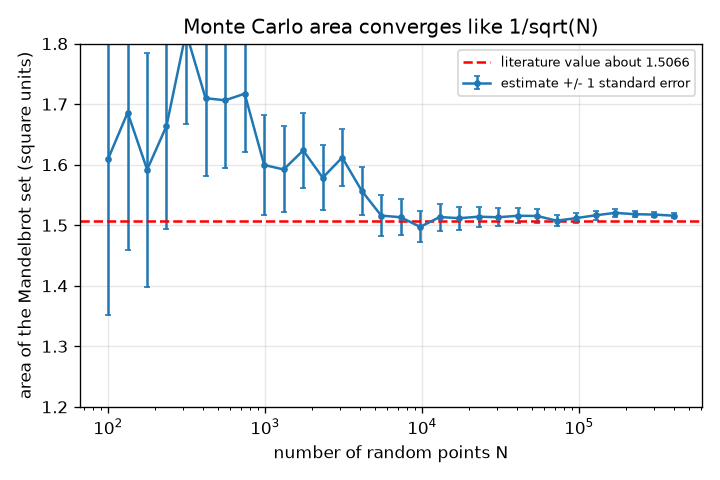
\includegraphics[width=0.85\linewidth]{figures/s03_area_convergence.png}\\\small Monte Carlo area estimate with error bars against the number of random points.\end{center}

\subsection*{E. Worked example}
For c = 1, find the integer count n with bailout 256, the escape value z\_n, and the smooth count nu by hand.
\begin{enumerate}[nosep]
\item The orbit of c = 1 is 0, 1, 2, 5, 26, 677, so the first value above 256 is z5 = 677 and n = 5.
\item ln 677 = 6.518.
\item log2(6.518) = ln 6.518 / ln 2 = 1.8745 / 0.6931 = 2.7044.
\item nu = n + 1 - log2(ln\textbar{}z\textbar{}) = 5 + 1 - 2.7044 = 3.296.
\end{enumerate}
\textbf{Answer.} n = 5, z5 = 677, nu = 3.296. (With the bailout 2 the integer count would be 3; the smooth count is built to agree between bailouts, up to a constant that we ignore in colouring.)

\subsection*{F. Questions}
\begin{enumerate}[nosep]
\item \textbf{Conceptual.} Why does the continuous count nu remove the colour bands, and why does it hardly depend on the bailout radius?
\item \textbf{Numerical.} A Monte Carlo run with N = 400,000 points gives a fraction p = 0.2631 inside the half-box. Give the area and the error bar. How many points would give an error bar half as large?
\item \textbf{Graph and simulation interpretation.} In the cost graph, why is the curve almost a straight line at a shallow zoom and bends over at a deep zoom?
\item \textbf{Design and optimisation challenge.} Design: you want a zoom video that stops at width 1e-13 and uses 200 pixel columns. Show that float64 is enough for the last frame and not for width 1e-15. Then propose what to do for the video to go to 1e-30.
\end{enumerate}

\section{Real-world mini-project}
\textbf{Find and render a mini-Mandelbrot.} Deep inside the picture, along the negative real axis, sits a small copy of the whole Mandelbrot set. Its centre is the real number c3 for which the orbit of 0 returns to 0 after exactly 3 steps. Use \texttt{period3\_centre} and \texttt{mislabelled} from Session 3 to locate it, render it, and find how many iterations a window of width 0.05 around it needs.

\section{The path ahead}
\begin{enumerate}[nosep]
\item \textbf{Session 4: Zoom beyond float64 with perturbation.} A deep-zoom renderer that keeps one high-precision orbit and perturbs around it.
\item \textbf{Session 5: Skip the interior.} A faster renderer that returns the same picture for the same window.
\item \textbf{Session 6: A better area estimate.} A second area estimator with a proper error bar.
\item \textbf{Session 7: A looping Julia morph.} A Julia-set animation as GIF or MP4 with c on a closed path.
\item \textbf{Session 8: Zoom video with automatic iterations.} A 120-frame zoom video that keeps the share of wrongly-inside pixels below 1 percent in every frame.
\end{enumerate}

\section{Answers and hints}

\subsection*{Session 1}
\begin{enumerate}[nosep]
\item \textbf{Conceptual.} Hint: Compute (a + b i) * i and compare the distances sqrt(a\textasciicircum{}2 + b\textasciicircum{}2) before and after. Solution: (a + b i) * i = a i + b i\textasciicircum{}2 = -b + a i, so the point (a, b) goes to (-b, a). The new distance is sqrt(b\textasciicircum{}2 + a\textasciicircum{}2), the same as before. The two points and 0 form a right angle (the vectors (a, b) and (-b, a) have dot product -ab + ab = 0), so it is a turn of 90 degrees counter-clockwise.
\item \textbf{Numerical.} Hint: Each step is 'square, then add 1'. Everything stays real. Solution: z1 = 1, z2 = 1\textasciicircum{}2 + 1 = 2, z3 = 2\textasciicircum{}2 + 1 = 5, z4 = 5\textasciicircum{}2 + 1 = 26. The distance is 1, 2, 5, 26: it is exactly 2 at step 2 (not above) and above 2 at step 3, so the orbit escapes at step 3. Sanity check: after the first escape the distances roughly square each time (5, 26, 677).
\item \textbf{Graph and simulation interpretation.} Hint: Compute z1, z2, z3 for c = -1. Solution: z1 = -1, z2 = (-1)\textasciicircum{}2 - 1 = 0, z3 = -1, z4 = 0 and so on: the distance alternates 1, 0, 1, 0 for ever (a cycle of length 2). It never reaches 2, so c = -1 stays. The graph is a zig-zag between 0 and 1, well below the red line.
\item \textbf{Design and optimisation challenge.} Hint: Use escape\_step(c, 50) in a loop over c = 0.20, 0.21, ... and over c = -1.90, -1.91, ... Solution: On the positive side c = 0.25 stays and c = 0.26 escapes (at step 30; the slow escapes close to 0.25 are why 50 steps is a rough test, see Session 2). On the negative side c = -2.00 stays and c = -2.01 escapes (at step 1). So the stay set on the real axis is a single interval from about -2 to 0.25. Assumption: 50 steps is enough; near the ends some c would need more steps, so the interval ends are approximate.
\end{enumerate}

\subsection*{Session 2}
\begin{enumerate}[nosep]
\item \textbf{Conceptual.} Hint: Think about which direction of the claim has a proof and which does not. Solution: Beyond 2 the distance grows by at least 3(\textbar{}z\textbar{} - 2) at every step, so the orbit can never come back: 'escapes' is a proof. 'Stays' after max\_iter steps only means 'has not escaped yet': orbits near the boundary can take very long, as c = 0.3 needs 12 steps and points near the boundary need hundreds. So the picture's inside is an upper bound on the real set that gets better with max\_iter.
\item \textbf{Numerical.} Hint: Squaring squares the modulus and doubles the argument. Solution: \textbar{}z\textasciicircum{}2\textbar{} = 25 and arg(z\textasciicircum{}2) = 2 * 53.13 = 106.26 degrees. Check: (3 + 4i)\textasciicircum{}2 = 9 + 24i + 16 i\textasciicircum{}2 = -7 + 24i; modulus sqrt(49 + 576) = 25; angle atan2(24, -7) = 106.26 degrees. Units: none (the arguments are in degrees).
\item \textbf{Graph and simulation interpretation.} Hint: Which pixels are wrongly inside, and where are they relative to the boundary? Solution: A pixel is wrongly inside if it escapes after max\_iter steps. Raising max\_iter lets more of them show their escape, so the error falls. A narrow window sits closer to the boundary where nearly every pixel is a slow escaper, so more of its pixels need long orbits: at max\_iter = 100 about 17 percent of the width-0.005 window is wrong, against 1.7 percent for width 0.5. The values are measured, not derived, and the reference at 1500 steps is itself approximate.
\item \textbf{Design and optimisation challenge.} Hint: Run smallest\_enough(SEAHORSE, width) for the two widths; try the same in-between. Solution: smallest\_enough gives 200 for width 0.5 (errors 0.7 percent at 200, 1.7 percent at 100) and 800 for width 0.005 (1.3 percent at 400 is too much, 0.1 percent at 800). For the video interpolate max\_iter on a log scale between 200 and 800 as the width shrinks, rounding up to the ladder. Trade-off: cost is roughly proportional to max\_iter wherever many pixels are inside, so 800 costs four times as much as 200 per frame; a cheaper choice accepts a few percent of smeared pixels. Assumption: the reference with 1500 steps is accurate enough.
\end{enumerate}

\subsection*{Session 3}
\begin{enumerate}[nosep]
\item \textbf{Conceptual.} Hint: Think about how \textbar{}z\textbar{} changes in the last step before and after crossing the bailout. Solution: Near escape the update z -\textgreater{} z\textasciicircum{}2 + c is dominated by z\textasciicircum{}2, so \textbar{}z\textbar{} roughly squares each step and ln\textbar{}z\textbar{} doubles; hence log2(ln\textbar{}z\textbar{}) increases by about 1 per step. The integer count n only changes in whole steps, but nu = n + 1 - log2(ln\textbar{}z\_n\textbar{}) subtracts the fraction of the last step by which \textbar{}z\_n\textbar{} overshot the bailout, so pixels that escape 'a little later' get a slightly larger nu. Changing the bailout from 256 to 10,000 changes n by about 1 and log2(ln\textbar{}z\textbar{}) by about 1 as well, so nu is nearly unchanged (differences below 1e-4 in the checkpoint).
\item \textbf{Numerical.} Hint: Use A = 2 * 2.875 * p and sigma = 2 * 2.875 * sqrt(p (1 - p) / N). Solution: A = 5.75 * 0.2631 = 1.513 (square units). sigma = 5.75 * sqrt(0.2631 * 0.7369 / 400000) = 5.75 * 0.000696 = 0.0040. The error scales like 1/sqrt(N), so halving it needs four times as many points, N = 1.6 million. Sanity check: the result agrees with 1.5066 within about 1.6 standard errors. (The run in lesson.py with max\_iter 2000 gives 1.5157 +/- 0.0040.)
\item \textbf{Graph and simulation interpretation.} Hint: Which pixels use all max\_iter steps, and which stop early? Solution: A pixel that stays inside uses all max\_iter steps, an escaping pixel uses only its escape count. If many pixels are inside, cost grows about proportionally to max\_iter (a straight line with slope = the number of inside pixels). When most pixels are outside and escape within a few hundred steps, raising max\_iter beyond their escape times adds no work, so the curve flattens (compare the full-set cost 2.8 million at 800 against 0.79 million at 200, with the seahorse window at width 0.01: 2.2 million against 1.5 million).
\item \textbf{Design and optimisation challenge.} Hint: Use distinct\_columns(SEAHORSE, width, 200) for several widths. Solution: At width 1e-13 all 200 columns have different coordinates, at 1e-14 only 91 do, at 1e-15 only 9 and at 1e-16 just 1, so float64 works down to about 1e-13 for 200 columns and then the picture turns into blocks. To go to 1e-30 you need more precision than 16 digits: arbitrary-precision numbers for one reference orbit and ordinary floats for the small differences from it (perturbation theory), which is the road to the Target. Trade-off: more digits cost more time per frame.
\end{enumerate}

\section{How to join}
Read \texttt{CONTRIBUTING.md} in the repository, then pick an issue labelled \texttt{good first issue}. Repository: \url{https://github.com/KrunalPanchal1995/openfractal}

\end{document}
